% !TeX program = xelatex
\documentclass[UTF8,a4paper,12pt]{ctexart}

\usepackage{amsmath,amssymb,amsthm,bm}
\usepackage{booktabs}
\usepackage{geometry}
\usepackage{enumitem}
\usepackage{listings}
\usepackage{xcolor}
\usepackage{graphicx}

\geometry{left=2.5cm,right=2.5cm,top=2.5cm,bottom=2.5cm}
\setlist[enumerate]{label=(\alph*),leftmargin=2em}
\setlist[itemize]{leftmargin=2em}
\lstset{
  basicstyle=\ttfamily\small,
  keywordstyle=\color{blue!60!black},
  commentstyle=\color{green!40!black},
  numbers=left,
  numberstyle=\tiny,
  frame=single,
  breaklines=true
}

\newcommand{\E}{\mathbb{E}}
\newcommand{\Var}{\operatorname{Var}}
\newcommand{\Cov}{\operatorname{Cov}}
\newcommand{\Prb}{\operatorname{Pr}}
\newcommand{\Normal}{\mathcal{N}}
\newcommand{\ind}{\mathbb{I}}

\title{《模式识别》课程作业（一）解答}
\author{}
\date{}

\begin{document}
\maketitle

\section*{第二章 数学背景知识}

\subsection*{习题 2.4}

将随机变量看作内积空间中的元素，定义
\[
    \langle X,Y\rangle=\E[XY].
\]
只要 $\E[X^2]$、$\E[Y^2]$ 有限，就有
\[
    0\le \E[(X-aY)^2]
      = \E[X^2]-2a\E[XY]+a^2\E[Y^2]
\]
对任意实数 $a$ 成立。若 $\E[Y^2]>0$，取
\[
    a=\frac{\E[XY]}{\E[Y^2]},
\]
代入得
\[
    0\le \E[X^2]-\frac{(\E[XY])^2}{\E[Y^2]}.
\]
因此
\[
    (\E[XY])^2\le \E[X^2]\E[Y^2].
\]
若 $\E[Y^2]=0$，则 $Y=0$ 几乎处处，$\E[XY]=0$，结论仍成立。这就是 Schwarz 不等式。

\subsection*{习题 2.5}

\begin{enumerate}
  \item 由协方差矩阵定义
  \[
      \Cov(X)=\E[(X-\E[X])(X-\E[X])^T].
  \]
  展开括号：
  \begin{align*}
      \Cov(X)
      &=\E\!\left[XX^T-X\E[X]^T-\E[X]X^T+\E[X]\E[X]^T\right]\\
      &=\E[XX^T]-\E[X]\E[X]^T-\E[X]\E[X]^T+\E[X]\E[X]^T\\
      &=\E[XX^T]-\E[X]\E[X]^T.
  \end{align*}

  \item 对常数 $u,v$，有
  \[
      \E[X+u]=\E[X]+u,\qquad \E[Y+v]=\E[Y]+v.
  \]
  因此
  \begin{align*}
      \Cov(X+u,Y+v)
      &=\E[((X+u)-\E[X+u])((Y+v)-\E[Y+v])^T]\\
      &=\E[(X-\E[X])(Y-\E[Y])^T]\\
      &=\Cov(X,Y).
  \end{align*}

  \item 对标量随机变量，相关系数为
  \[
      \rho_{X,Y}=\frac{\Cov(X,Y)}{\sigma_X\sigma_Y}.
  \]
  令 $\tilde X=X-\E[X]$，$\tilde Y=Y-\E[Y]$。由 Schwarz 不等式，
  \[
      \Cov(X,Y)^2=(\E[\tilde X\tilde Y])^2
      \le \E[\tilde X^2]\E[\tilde Y^2]
      =\sigma_X^2\sigma_Y^2.
  \]
  若 $\sigma_X\sigma_Y>0$，两边除以 $\sigma_X^2\sigma_Y^2$，得
  \[
      \rho_{X,Y}^2\le 1,
  \]
  即
  \[
      -1\le \rho_{X,Y}\le 1.
  \]
  若某个标准差为 $0$，相关系数通常不定义；在非退化情形下上式成立。
\end{enumerate}

\section*{第四章 评估}

\subsection*{习题 4.1}

已知正例数 $P=100$、负例数 $N=100$。由
\[
    \mathrm{TPR}=\frac{TP}{P}=0.2,\qquad
    \mathrm{FPR}=\frac{FP}{N}=0.3,
\]
得到
\[
    TP=20,\quad FN=80,\quad FP=30,\quad TN=70.
\]
所以
\[
    \mathrm{Precision}=\frac{TP}{TP+FP}
      =\frac{20}{20+30}=0.4,
\]
\[
    \mathrm{Recall}=\frac{TP}{TP+FN}
      =\frac{20}{100}=0.2.
\]
于是
\[
    F_1=\frac{2TP}{2TP+FP+FN}
      =\frac{40}{40+30+80}
      =\frac{4}{15}\approx 0.2667.
\]
准确率和错误率分别为
\[
    \mathrm{Accuracy}=\frac{TP+TN}{P+N}
      =\frac{20+70}{200}=0.45,
\]
\[
    \mathrm{Error\ Rate}=1-\mathrm{Accuracy}=0.55.
\]

\subsection*{习题 4.5}

把类别 $1$ 看作正类。按照得分从高到低排序后，逐步把样本判为正例。共有 $5$ 个正例，因此
\[
    r_i=\frac{TP_i}{5},\qquad p_i=\frac{TP_i}{i}.
\]
取 $(r_0,p_0)=(0,1)$。

\begin{center}
\begin{tabular}{cccccc}
\toprule
$i$ & 类别 & 得分 & $TP_i$ & $p_i$ & $r_i$\\
\midrule
0 & -- & --  & 0 & 1.0000 & 0.0000\\
1 & 1  & 1.0 & 1 & 1.0000 & 0.2000\\
2 & 2  & 0.9 & 1 & 0.5000 & 0.2000\\
3 & 1  & 0.8 & 2 & 0.6667 & 0.4000\\
4 & 1  & 0.7 & 3 & 0.7500 & 0.6000\\
5 & 2  & 0.6 & 3 & 0.6000 & 0.6000\\
6 & 1  & 0.5 & 4 & 0.6667 & 0.8000\\
7 & 2  & 0.4 & 4 & 0.5714 & 0.8000\\
8 & 2  & 0.3 & 4 & 0.5000 & 0.8000\\
9 & 1  & 0.2 & 5 & 0.5556 & 1.0000\\
10& 2  & 0.1 & 5 & 0.5000 & 1.0000\\
\bottomrule
\end{tabular}
\end{center}

\begin{enumerate}
  \item 梯形法计算
  \[
      \mathrm{AUC\text{-}PR}
      =\sum_{i=1}^{10}(r_i-r_{i-1})\frac{p_i+p_{i-1}}{2}.
  \]
  只有召回率变化的位置有贡献，即 $i=1,3,4,6,9$：
  \begin{align*}
      \mathrm{AUC\text{-}PR}
      &=0.2\cdot\frac{1+1}{2}
        +0.2\cdot\frac{0.6667+0.5}{2}\\
      &\quad+0.2\cdot\frac{0.75+0.6667}{2}
        +0.2\cdot\frac{0.6667+0.6}{2}\\
      &\quad+0.2\cdot\frac{0.5556+0.5}{2}\\
      &\approx 0.6906.
  \end{align*}

  \item AP 使用矩形法：
  \[
      \mathrm{AP}=\sum_{i=1}^{10}(r_i-r_{i-1})p_i.
  \]
  因此
  \[
      \mathrm{AP}
      =0.2(1+0.6667+0.75+0.6667+0.5556)
      \approx 0.7278.
  \]
  AUC-PR 使用相邻两点精度的平均值，AP 使用当前点精度作为高度；所以两者都是 PR 曲线的面积型总结，但插值方式不同。

  \item 若交换第 9 行和第 10 行的类别标记，则最后两个样本类别变为 $2,1$。正例仍有 $5$ 个，但最后一个正例的排名更靠后。重新计算得到
  \[
      \mathrm{AUC\text{-}PR}\approx 0.6794,\qquad
      \mathrm{AP}\approx 0.7167.
  \]
  两个值都降低，说明 AUC-PR 和 AP 对正例排序位置敏感：正例越靠前，曲线面积越大。

  \item 可用如下程序验证：
\begin{lstlisting}[language=Python]
labels = [1, 2, 1, 1, 2, 1, 2, 2, 1, 2]
scores = [1.0, .9, .8, .7, .6, .5, .4, .3, .2, .1]
order = sorted(range(len(scores)), key=lambda i: -scores[i])
P = sum(labels[i] == 1 for i in order)

r = [0.0]
p = [1.0]
tp = 0
for t, i in enumerate(order, start=1):
    tp += int(labels[i] == 1)
    r.append(tp / P)
    p.append(tp / t)

auc_pr = sum((r[i] - r[i-1]) * (p[i] + p[i-1]) / 2
             for i in range(1, len(r)))
ap = sum((r[i] - r[i-1]) * p[i]
         for i in range(1, len(r)))
print(auc_pr, ap)
\end{lstlisting}
  输出约为 $0.6906$ 和 $0.7278$，与手算一致。
\end{enumerate}

\subsection*{习题 4.6}

测试点 $x$ 的真实标记为
\[
    y=F(x)+\epsilon,\qquad \E[\epsilon]=0,\qquad \Var(\epsilon)=\sigma^2.
\]
k-NN 回归预测为
\[
    f(x;D)=\frac{1}{k}\sum_{i=1}^k y_{nn(i)}.
\]

\begin{enumerate}
  \item 对固定 $x$，记
  \[
      \bar f(x)=\E_D[f(x;D)].
  \]
  则
  \begin{align*}
      \E[(y-f(x;D))^2]
      &=\E[(F(x)+\epsilon-f(x;D))^2]\\
      &=\E[(F(x)-f(x;D))^2]+\E[\epsilon^2]\\
      &=\E_D[(F(x)-f(x;D))^2]+\sigma^2.
  \end{align*}
  在第一项中加减 $\bar f(x)$：
  \begin{align*}
      \E_D[(F(x)-f(x;D))^2]
      &=\E_D[(F(x)-\bar f(x)+\bar f(x)-f(x;D))^2]\\
      &=(F(x)-\bar f(x))^2+\E_D[(f(x;D)-\bar f(x))^2],
  \end{align*}
  因为交叉项期望为 $0$。因此
  \[
      \E[(y-f(x;D))^2]
      =
      \underbrace{(F(x)-\E_D[f(x;D)])^2}_{\text{偏差平方}}
      +
      \underbrace{\E_D[(f(x;D)-\E_D[f(x;D)])^2]}_{\text{方差}}
      +
      \underbrace{\sigma^2}_{\text{不可约噪声}}.
  \]

  \item 由 $y_{nn(i)}=F(x_{nn(i)})+\epsilon_{nn(i)}$，且噪声均值为 $0$，
  \[
      \E_D[f(x;D)]
      =
      \E_D\left[\frac{1}{k}\sum_{i=1}^k y_{nn(i)}\right]
      =
      \frac{1}{k}\sum_{i=1}^k \E_D[F(x_{nn(i)})].
  \]
  若训练样本充分密集，$x_{nn(i)}$ 接近 $x$，则该值近似为 $F(x)$。

  \item 将 k-NN 的具体表达式代入偏差--方差分解。由上一问
  \[
      \E_D[f(x;D)]
      =
      \E_D\left[\frac{1}{k}\sum_{i=1}^k y_{nn(i)}\right]
      =
      \frac{1}{k}\sum_{i=1}^k \E_D[F(x_{nn(i)})],
  \]
  因此偏差平方项为
  \[
      \left(
      F(x)-
      \frac{1}{k}\sum_{i=1}^k \E_D[F(x_{nn(i)})]
      \right)^2.
  \]
  方差项为
  \[
      \E_D\left[
      \left(
      \frac{1}{k}\sum_{i=1}^k y_{nn(i)}
      -
      \E_D\left[\frac{1}{k}\sum_{i=1}^k y_{nn(i)}\right]
      \right)^2
      \right].
  \]
  代入 $y_{nn(i)}=F(x_{nn(i)})+\epsilon_{nn(i)}$，可进一步写成
  \[
      \E_D\left[
      \left(
      \frac{1}{k}\sum_{i=1}^k
      \bigl(F(x_{nn(i)})+\epsilon_{nn(i)}\bigr)
      -
      \frac{1}{k}\sum_{i=1}^k \E_D[F(x_{nn(i)})]
      \right)^2
      \right].
  \]
  所以完整误差为
  \[
      \E[(y-f(x;D))^2]
      =
      \left(
      F(x)-
      \frac{1}{k}\sum_{i=1}^k \E_D[F(x_{nn(i)})]
      \right)^2
      +\Var_D\!\left(
      \frac{1}{k}\sum_{i=1}^k y_{nn(i)}
      \right)
      +\sigma^2.
  \]

  \item 若近邻位置固定且只考虑观测噪声，则
  \[
      \Var(f(x;D))=\Var\left(\frac{1}{k}\sum_{i=1}^k \epsilon_{nn(i)}\right)
      =\frac{\sigma^2}{k}.
  \]
  更一般地还包含近邻位置随机带来的波动。随着 $k$ 增大，平均会降低方差，所以方差项通常减小。

  \item 偏差平方项是
  \[
      \mathrm{Bias}^2(x)
      =
      \left(
      F(x)-
      \E_D[f(x;D)]
      \right)^2
      =
      \left(
      F(x)-
      \frac{1}{k}\sum_{i=1}^k \E_D[F(x_{nn(i)})]
      \right)^2.
  \]
  $k$ 增大时，预测会对更大范围的邻居取平均。若 $F$ 在 $x$ 附近不是常数，则较远邻居的函数值 $F(x_{nn(i)})$ 与 $F(x)$ 的差异通常更大，所以偏差平方通常增大。极端情形 $k=n$ 时，
  \[
      f(x;D)=\frac{1}{n}\sum_{i=1}^n y_i
  \]
  与 $x$ 无关，是一个全局常数模型。此时
  \[
      \E_D[f(x;D)]
      =
      \frac{1}{n}\sum_{i=1}^n \E_D[F(x_i)]
  \]
  是全局平均意义下的回归函数值，因此
  \[
      \mathrm{Bias}^2(x)
      =
      \left(
      F(x)-\frac{1}{n}\sum_{i=1}^n \E_D[F(x_i)]
      \right)^2.
  \]
  除非 $F(x)$ 本身接近这个全局平均，否则该偏差会较大。
\end{enumerate}

\subsection*{习题 4.7}

已知
\[
    p(x\mid y=1)=\Normal(-1,0.25),\qquad
    p(x\mid y=2)=\Normal(1,0.25),
\]
\[
    \Prb(y=1)=\Prb(y=2)=0.5.
\]

\begin{enumerate}
  \item 由全概率公式，
  \[
      p(x)=\sum_{y=1}^2p(x\mid y)\Prb(y)
      =\frac{1}{2}\Normal(x\mid -1,0.25)
       +\frac{1}{2}\Normal(x\mid 1,0.25).
  \]
  写成显式形式为
  \[
      p(x)=\frac{1}{2\sqrt{2\pi\cdot0.25}}
      \left[
      \exp\!\left(-\frac{(x+1)^2}{2\cdot0.25}\right)
      +
      \exp\!\left(-\frac{(x-1)^2}{2\cdot0.25}\right)
      \right].
  \]

  \item 对 $0$-$1$ 损失矩阵
  \[
      C=\begin{pmatrix}0&1\\1&0\end{pmatrix},
  \]
  条件风险为
  \[
      R(\hat y=1\mid x)=\Prb(y=2\mid x),\qquad
      R(\hat y=2\mid x)=\Prb(y=1\mid x).
  \]
  因此最小化条件风险等价于选择后验概率最大的类别：
  \[
      f(x)=\arg\max_y p(y\mid x).
  \]
  对任意 $x$，这样选择都使条件风险最小，所以它是 Bayes 最优分类器。
  在多分类 $0$-$1$ 损失下，同理有
  \[
      R(\hat y=j\mid x)=1-p(y=j\mid x),
  \]
  因而仍应选择后验概率最大的类别。所以该规则在多分类 $0$-$1$ 损失下也是最优的。

  \item 本题中两类先验相同、方差相同，Bayes 分类只需比较两个类条件密度。分界点满足
  \[
      \Normal(x\mid -1,0.25)=\Normal(x\mid 1,0.25),
  \]
  即
  \[
      (x+1)^2=(x-1)^2,
  \]
  得 $x=0$。所以最优策略为
  \[
      f(x)=
      \begin{cases}
      1, & x<0,\\
      2, & x\ge 0.
      \end{cases}
  \]
  其错误率为
  \[
      \frac{1}{2}\Prb_{X\sim\Normal(-1,0.25)}(X\ge0)
      +\frac{1}{2}\Prb_{X\sim\Normal(1,0.25)}(X<0)
      =\Phi(-2)\approx 0.0228.
  \]

  \item 新损失矩阵为
  \[
      C=\begin{pmatrix}0&10\\1&0\end{pmatrix},
  \]
  其中真实类别为 $1$ 却预测为 $2$ 的代价为 $10$。条件风险为
  \[
      R(\hat y=1\mid x)=\Prb(y=2\mid x),
  \]
  \[
      R(\hat y=2\mid x)=10\Prb(y=1\mid x).
  \]
  因此选择类别 $1$ 当且仅当
  \[
      \Prb(y=2\mid x)<10\Prb(y=1\mid x),
  \]
  等价于
  \[
      \frac{p(x\mid y=2)}{p(x\mid y=1)}<10.
  \]
  两类方差均为 $0.25$，所以
  \[
      \log\frac{p(x\mid y=2)}{p(x\mid y=1)}
      =-\frac{(x-1)^2-(x+1)^2}{2\cdot0.25}
      =8x.
  \]
  因而阈值满足
  \[
      8x<\log 10.
  \]
  新规则为
  \[
      f(x)=
      \begin{cases}
      1, & x<\dfrac{\log 10}{8},\\[4pt]
      2, & x\ge \dfrac{\log 10}{8}.
      \end{cases}
  \]
  阈值约为 $0.2878$，比 $0$-$1$ 损失下的阈值右移，因为把类别 $1$ 错分成类别 $2$ 的代价更大。
\end{enumerate}

\section*{第六章 Fisher 线性判别}

\subsection*{习题 6.5}

设共有 $C>2$ 类，样本维数为 $D$，总样本数为 $N$。类内散度矩阵为 $S_W$，类间散度矩阵为 $S_B$。

\begin{enumerate}
  \item 对第 $k$ 类，类内散度的秩至多为 $N_k-1$，因为该类样本减去类均值后向量和为 $0$。因此
  \[
      \operatorname{rank}(S_W)
      \le \sum_{k=1}^C (N_k-1)
      =N-C.
  \]
  若 $N<D$，则
  \[
      \operatorname{rank}(S_W)\le N-C<D,
  \]
  所以 $S_W$ 必然不可逆。

  \item 类间散度矩阵为
  \[
      S_B=\sum_{k=1}^C N_k(m_k-m)(m_k-m)^T.
  \]
  它的列空间由 $C$ 个向量 $m_k-m$ 张成。但这些向量满足加权和为零：
  \[
      \sum_{k=1}^C N_k(m_k-m)=0.
  \]
  因而它们至多张成 $C-1$ 维空间，所以
  \[
      \operatorname{rank}(S_B)\le C-1.
  \]
  FLD 最多只能获得 $C-1$ 个有效特征向量。

  \item 当 $N>D$，尤其 $N\gg D$ 时，$\operatorname{rank}(S_W)\le D$ 不再强迫 $S_W$ 奇异。若各类样本在特征空间中的类内变化能够张成整个 $\mathbb{R}^D$，则 $S_W$ 可满秩，从而可逆。不过这不是必然的；若样本存在严格线性相关或某些维度没有类内变化，$S_W$ 仍可能奇异。

  \item 假设 $S_W$ 正定，Cholesky 分解为
  \[
      S_W=GG^T.
  \]
  令
  \[
      C=G^{-1}S_BG^{-T}.
  \]
  若 $Q$ 为正交矩阵，使
  \[
      Q^TCQ=\Lambda
  \]
  为对角矩阵，并令
  \[
      X=G^{-T}Q,
  \]
  记
  \[
      Q=[q_1,\ldots,q_D],\qquad
      X=[x_1,\ldots,x_D],
  \]
  则
  \[
      x_j=G^{-T}q_j.
  \]

  首先证明 $X^TS_WX$ 是单位矩阵：
  \[
      X^TS_WX
      =Q^TG^{-1}GG^TG^{-T}Q
      =Q^TQ=I.
  \]
  其次证明 $X^TS_BX$ 是对角矩阵：
  \[
      X^TS_BX
      =Q^TG^{-1}S_BG^{-T}Q
      =Q^TCQ
      =\Lambda,
  \]
  其中 $\Lambda=\operatorname{diag}(\lambda_1,\ldots,\lambda_D)$。
  因而 $X^TS_BX$ 的对角线元素就是 $\lambda_1,\ldots,\lambda_D$。

  再证明 $X$ 的列向量是广义特征向量。由于
  \[
      Cq_j=\lambda_j q_j,
  \]
  即
  \[
      G^{-1}S_BG^{-T}q_j=\lambda_jq_j.
  \]
  由 $x_j=G^{-T}q_j$ 和 $q_j=G^Tx_j$，上式可写为
  \[
      G^{-1}S_Bx_j=\lambda_jG^Tx_j.
  \]
  两边左乘 $G$，得到
  \[
      S_Bx_j=\lambda_jGG^Tx_j=\lambda_jS_Wx_j.
  \]
  所以 $x_j$ 正是广义特征值问题
  \[
      S_Bw=\lambda S_Ww
  \]
  的广义特征向量，广义特征值为 $\lambda_j$。因此，广义特征向量位于 $X$ 的列中，广义特征值位于 $X^TS_BX=\Lambda$ 的对角线上。

  由于 $\operatorname{rank}(S_B)\le C-1$，非零广义特征值最多有 $C-1$ 个，所以有效判别方向最多为 $C-1$ 个。

  最后讨论单位范数和正交性。由
  \[
      X^TS_WX=I
  \]
  可得
  \[
      x_i^TS_Wx_j=
      \begin{cases}
      1,& i=j,\\
      0,& i\ne j.
      \end{cases}
  \]
  因而这些向量在 $S_W$ 诱导的内积下是单位正交的，也就是具有 $S_W$-单位范数。但它们在普通欧氏意义下不一定有单位范数，因为
  \[
      X^TX=Q^TG^{-1}G^{-T}Q\ne I,
  \]
  一般不能推出 $x_j^Tx_j=1$。同理，它们在普通欧氏内积下也不一定正交；只能保证关于 $S_W$ 的广义正交性。
\end{enumerate}

\subsection*{习题 6.6}

本实验使用 ORL/AT\&T 人脸数据集。数据集中共有 $40$ 个类别，每个类别对应一个人，每人 $10$ 张灰度人脸图像。因此总样本数为
\[
    N=400.
\]
每张图像大小为 $112\times92$，将图像按像素展开后，每个人脸样本可表示为高维向量
\[
    x_i\in\mathbb{R}^{112\times92}.
\]
实验中按类别分层划分训练集和测试集，其中训练集大小为 $240$，测试集大小为 $160$。

\begin{enumerate}
  \item Eigenfaces 方法基于 PCA。首先计算平均脸
  \[
      \bar x=\frac{1}{N}\sum_{i=1}^N x_i,
  \]
  然后对中心化样本 $x_i-\bar x$ 做主成分分析。主成分方向可以重新排列成人脸图像，称为 eigenfaces。测试样本 $x$ 投影到 PCA 子空间中得到
  \[
      z=W_{\mathrm{PCA}}^T(x-\bar x).
  \]
  本实验中 Eigenfaces 使用 $80$ 个主成分。实验得到识别准确率为
  \[
      \mathrm{Accuracy}_{\mathrm{Eigenfaces}}=0.9437.
  \]
  由于测试集共有 $160$ 张图像，该结果约等于正确识别 $151$ 张人脸。

  \item Fisherfaces 方法基于 FLD。它利用类别标记，希望投影后类内散度尽可能小、类间散度尽可能大，即最大化
  \[
      J(W)=\frac{|W^TS_BW|}{|W^TS_WW|}.
  \]
  由于人脸图像维数远大于训练样本数，直接求 FLD 时 $S_W$ 容易奇异，因此实际 Fisherfaces 通常先通过 PCA 降维，再在 PCA 子空间中做 FLD。ORL 数据集中共有 $C=40$ 类，所以 FLD 最多得到 $C-1=39$ 个有效判别方向。本实验中 Fisherfaces 使用 $39$ 个判别方向，识别准确率为
  \[
      \mathrm{Accuracy}_{\mathrm{Fisherfaces}}=0.9125.
  \]
  对 $160$ 张测试图像而言，该结果对应正确识别 $146$ 张人脸。

  \item 两种方法的实验结果如下：
  \[
      \mathrm{Accuracy}_{\mathrm{Eigenfaces}}=94.37\%,
      \qquad
      \mathrm{Accuracy}_{\mathrm{Fisherfaces}}=91.25\%.
  \]
  在本次训练测试划分和参数设置下，Eigenfaces 的准确率高于 Fisherfaces，差值约为
  \[
      94.37\%-91.25\%=3.12\%.
  \]
  这说明实际识别效果不仅取决于方法本身，也受到训练测试划分、样本数量、保留维数和模型实现的影响。理论上，Fisherfaces 利用类别标记，更直接优化分类可分性；但在小样本情况下，FLD 对训练数据划分较敏感，若估计得到的类内散度和类间散度不够稳定，测试集表现可能不如 Eigenfaces。

  \item 从生成的平均脸和 eigenfaces 图像可以观察到，平均脸保留了 ORL 数据集中人脸的大致轮廓、眼睛、鼻子和嘴的位置，但由于所有人的差异被平均掉，图像较模糊。前若干个 eigenfaces 不是普通人脸图像，而是一些明暗变化模式，主要反映训练集中方差最大的方向，例如整体光照变化、脸部轮廓变化和局部阴影变化。这与 PCA 的目标一致：PCA 保留的是总体方差最大的方向，而不是直接针对分类错误率优化。

  \begin{figure}[htbp]
      \centering
      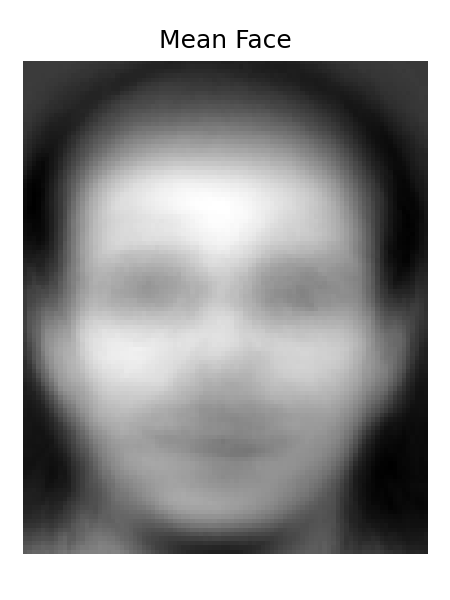
\includegraphics[width=0.35\textwidth]{6_6/mean_face.png}
      \caption{ORL 数据集平均脸}
  \end{figure}

  \begin{figure}[htbp]
      \centering
      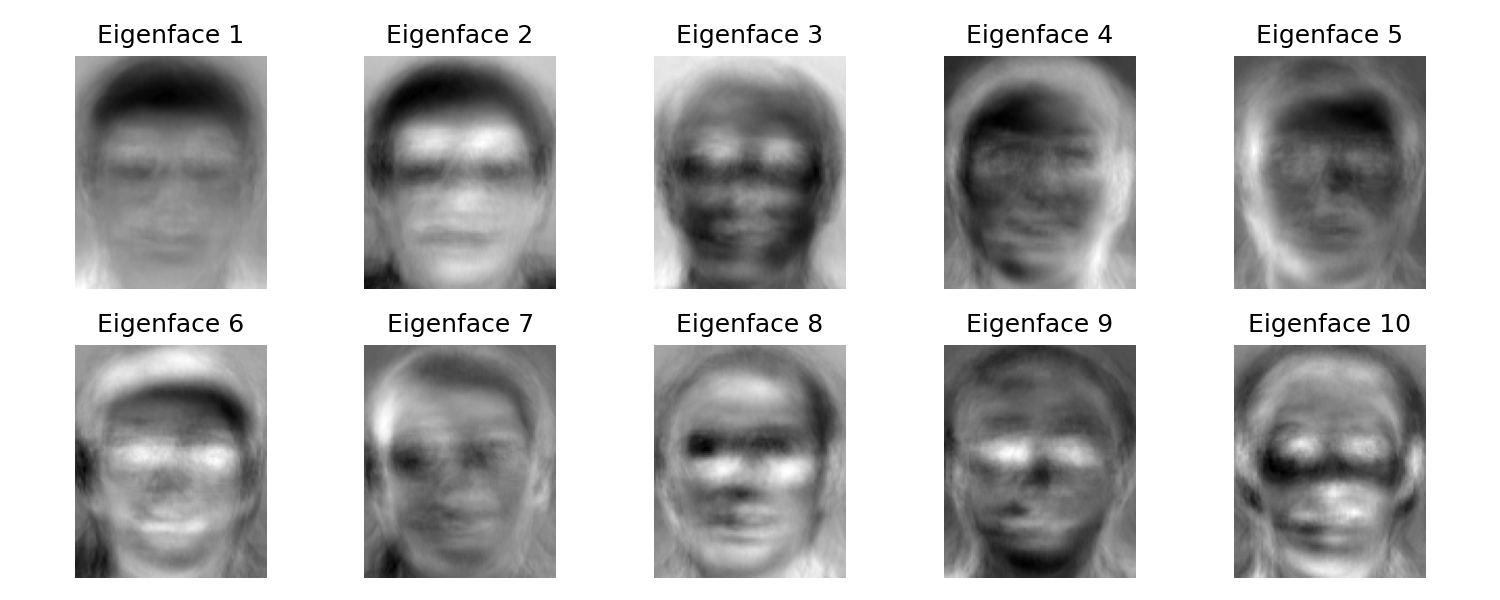
\includegraphics[width=0.90\textwidth]{6_6/top10_eigenfaces.png}
      \caption{前 10 个 eigenfaces}
  \end{figure}

  \item Eigenfaces 还可以用于人脸重构。若使用前 $r$ 个 eigenfaces $u_1,\ldots,u_r$，则人脸 $x$ 的重构为
  \[
      \hat x=\bar x+\sum_{j=1}^r a_j u_j,
      \qquad a_j=u_j^T(x-\bar x).
  \]
  实验中随着 $r$ 增大，重构图像逐渐接近原始人脸。使用较少 eigenfaces 时，重构图像只能保留大致脸型和低频结构，五官细节较模糊；使用更多 eigenfaces 后，眼睛、鼻子、嘴部轮廓等个体细节逐渐恢复。这说明 PCA 主成分数量越多，保留的信息越多，重构误差越小。

  \begin{figure}[htbp]
      \centering
      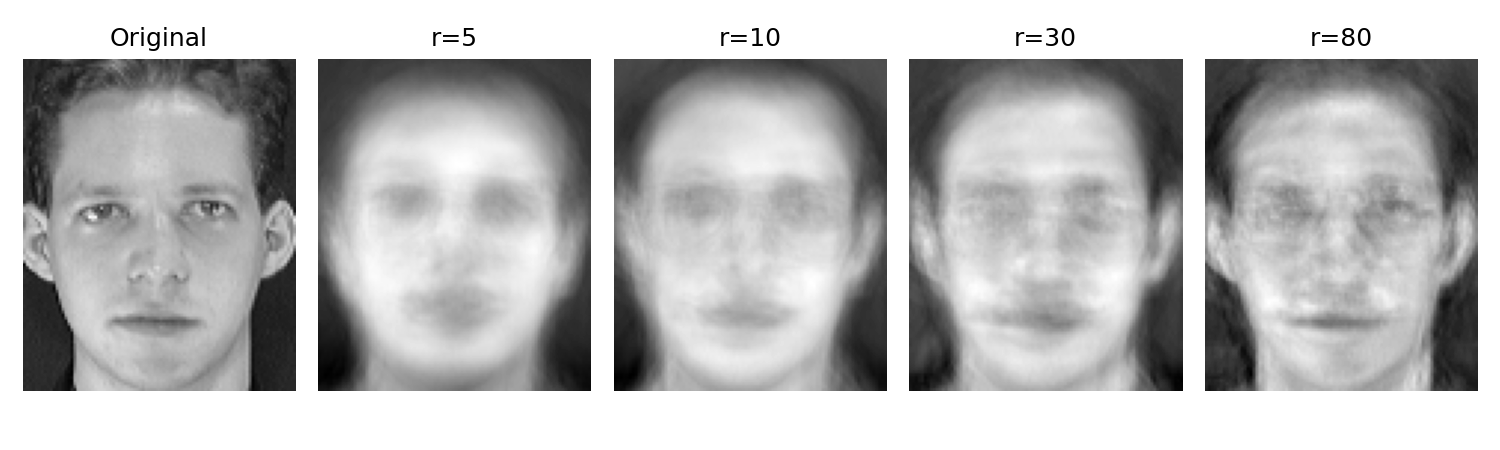
\includegraphics[width=0.32\textwidth]{6_6/reconstruction_0.png}
      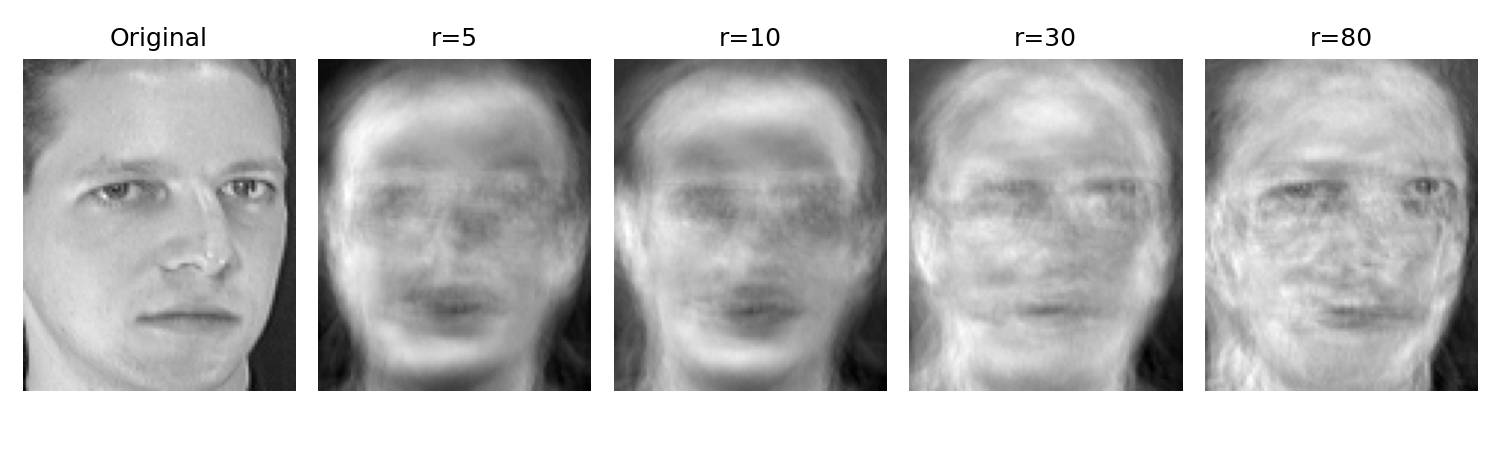
\includegraphics[width=0.32\textwidth]{6_6/reconstruction_1.png}
      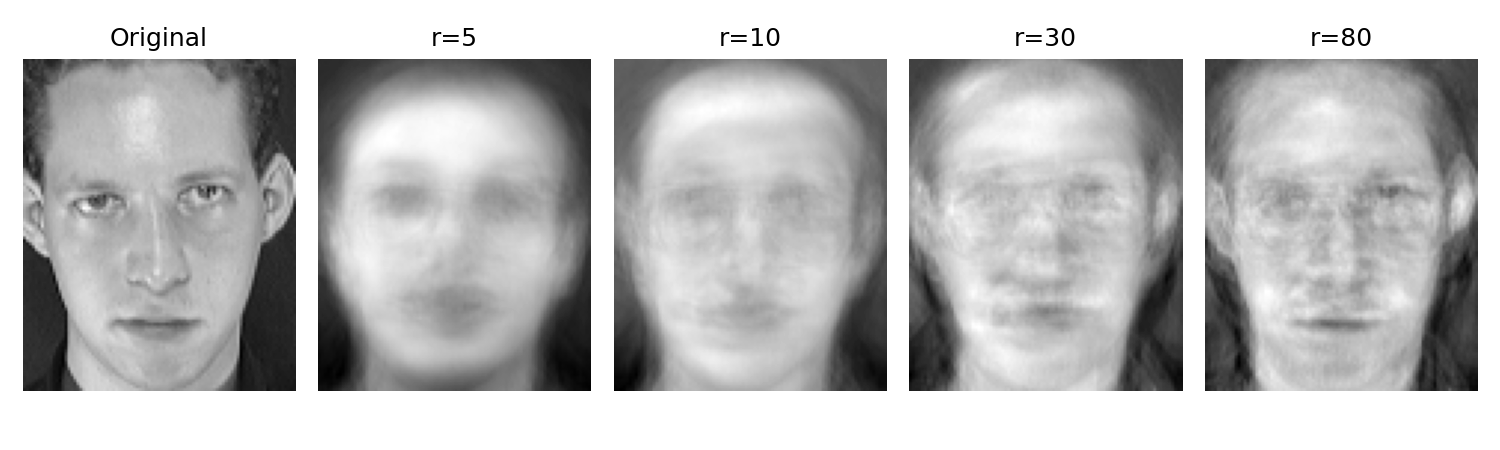
\includegraphics[width=0.32\textwidth]{6_6/reconstruction_2.png}
      \caption{不同样本人脸在不同 eigenfaces 数量下的重构结果}
  \end{figure}

  \item 综合来看，Eigenfaces 更强调对人脸图像整体变化的表达和重构，Fisherfaces 更强调类别之间的判别能力。本次实验中 Eigenfaces 的识别率更高，说明在该训练测试划分和参数设置下，PCA 保留的主要变化方向已经能够较好地区分 ORL 中的人脸类别；而 Fisherfaces 虽然具有判别性，但在样本数较少时对估计和划分更敏感。因此，实际应用中需要通过交叉验证选择 PCA 维数、FLD 维数和分类策略，而不能只根据理论性质判断哪一种方法一定更优。
\end{enumerate}

\section*{第八章 概率方法}

\subsection*{习题 8.1}

指数分布密度为
\[
    p(x;\lambda)=\lambda e^{-\lambda x}\ind[x\ge0],\qquad \lambda>0.
\]
对独立样本 $D=\{x_1,\ldots,x_n\}$，若所有 $x_i\ge0$，似然为
\[
    L(\lambda)=\prod_{i=1}^n \lambda e^{-\lambda x_i}
    =\lambda^n\exp\!\left(-\lambda\sum_{i=1}^n x_i\right).
\]
对数似然为
\[
    \ell(\lambda)=n\log\lambda-\lambda\sum_{i=1}^n x_i.
\]
求导得
\[
    \frac{\partial \ell}{\partial\lambda}
    =\frac{n}{\lambda}-\sum_{i=1}^n x_i.
\]
令其为 $0$，
\[
    \hat\lambda_{\mathrm{MLE}}
    =\frac{n}{\sum_{i=1}^n x_i}
    =\frac{1}{\bar x}.
\]
二阶导数 $-n/\lambda^2<0$，所以该驻点为最大值。

\subsection*{习题 8.2}

Pareto 分布密度为
\[
    p(x)=\frac{\alpha x_m^\alpha}{x^{\alpha+1}}\ind[x\ge x_m],
    \qquad x_m>0,\ \alpha>0.
\]

\begin{enumerate}
  \item 若
  \[
      p_1(x)=\frac{c_1}{x^{\alpha+1}}\ind[x\ge x_m],
  \]
  则归一化要求
  \[
      1=\int_{x_m}^{\infty}\frac{c_1}{x^{\alpha+1}}\,dx
      =c_1\frac{x_m^{-\alpha}}{\alpha}.
  \]
  因此
  \[
      c_1=\alpha x_m^\alpha.
  \]
  所以 $X\sim\mathrm{Pareto}(x_m,\alpha)$。

  \item 对 $D=\{x_1,\ldots,x_n\}$，似然为
  \[
      L(x_m,\alpha)
      =\prod_{i=1}^n
      \frac{\alpha x_m^\alpha}{x_i^{\alpha+1}}\ind[x_i\ge x_m].
  \]
  记 $x_{(1)}=\min_i x_i$。若 $x_m\le x_{(1)}$，
  \[
      \ell(x_m,\alpha)
      =n\log\alpha+n\alpha\log x_m-(\alpha+1)\sum_{i=1}^n\log x_i.
  \]
  固定 $x_m$，对 $\alpha$ 求导：
  \[
      \frac{\partial\ell}{\partial\alpha}
      =\frac{n}{\alpha}+n\log x_m-\sum_{i=1}^n\log x_i.
  \]
  因而
  \[
      \hat\alpha(x_m)
      =
      \frac{n}{\sum_{i=1}^n\log(x_i/x_m)}.
  \]
  对 $x_m$ 而言，在约束 $x_m\le x_{(1)}$ 下，似然随 $x_m$ 增大而增大，因此
  \[
      \hat x_m=x_{(1)}=\min_i x_i.
  \]
  于是
  \[
      \hat\alpha
      =
      \frac{n}{\sum_{i=1}^n\log(x_i/\hat x_m)}.
  \]

  \item 若
  \[
      x_i\mid \theta\sim \mathrm{Uniform}(0,\theta),
  \]
  则似然为
  \[
      p(D\mid \theta)=\theta^{-n}\ind[\theta\ge x_{(n)}],
  \]
  其中 $x_{(n)}=\max_i x_i$。若先验为
  \[
      \theta\sim\mathrm{Pareto}(x_m,k),
  \]
  即
  \[
      p(\theta)=\frac{kx_m^k}{\theta^{k+1}}\ind[\theta\ge x_m],
  \]
  则后验满足
  \[
      p(\theta\mid D)
      \propto
      \theta^{-n}\ind[\theta\ge x_{(n)}]\cdot
      \theta^{-(k+1)}\ind[\theta\ge x_m].
  \]
  因此
  \[
      p(\theta\mid D)
      \propto
      \theta^{-(n+k+1)}
      \ind[\theta\ge \max(x_m,x_{(n)})].
  \]
  这仍是 Pareto 分布：
  \[
      \theta\mid D\sim
      \mathrm{Pareto}\bigl(\max(x_m,x_{(n)}),\,k+n\bigr).
  \]
  所以 Pareto 先验是该均匀分布上界参数问题的共轭先验。
\end{enumerate}

\subsection*{习题 8.4}

对数正态分布为
\[
    p(x)=
    \begin{cases}
    \dfrac{1}{\sqrt{2\pi}\sigma x}
    \exp\!\left[-\dfrac{(\ln x-\mu)^2}{2\sigma^2}\right],
    & x>0,\\[6pt]
    0,& x\le0.
    \end{cases}
\]
本题中 $\mu=2,\sigma=0.5$。

\begin{enumerate}
  \item 从该分布生成 $1000$ 个独立样本。实验中得到样本均值和样本方差为
  \[
      \bar x=8.119600,\qquad s^2=17.360589.
  \]
  理论均值和方差分别为
  \[
      \E[X]=\exp\!\left(\mu+\frac{\sigma^2}{2}\right)
      =\exp(2.125)\approx 8.372897,
  \]
  \[
      \Var(X)=\left(\exp(\sigma^2)-1\right)\exp(2\mu+\sigma^2)
      \approx 19.911719.
  \]
  真实密度曲线在 $x>0$ 上先上升后下降，峰值位置为
  \[
      \operatorname{mode}(X)=\exp(\mu-\sigma^2)=\exp(1.75)\approx 5.7546.
  \]
  实验结果中样本均值和方差与理论值接近。因为对数正态分布右尾较长，所以样本直方图在 $5$ 到 $10$ 附近较密集，并向右拖出长尾。

  \begin{figure}[htbp]
      \centering
      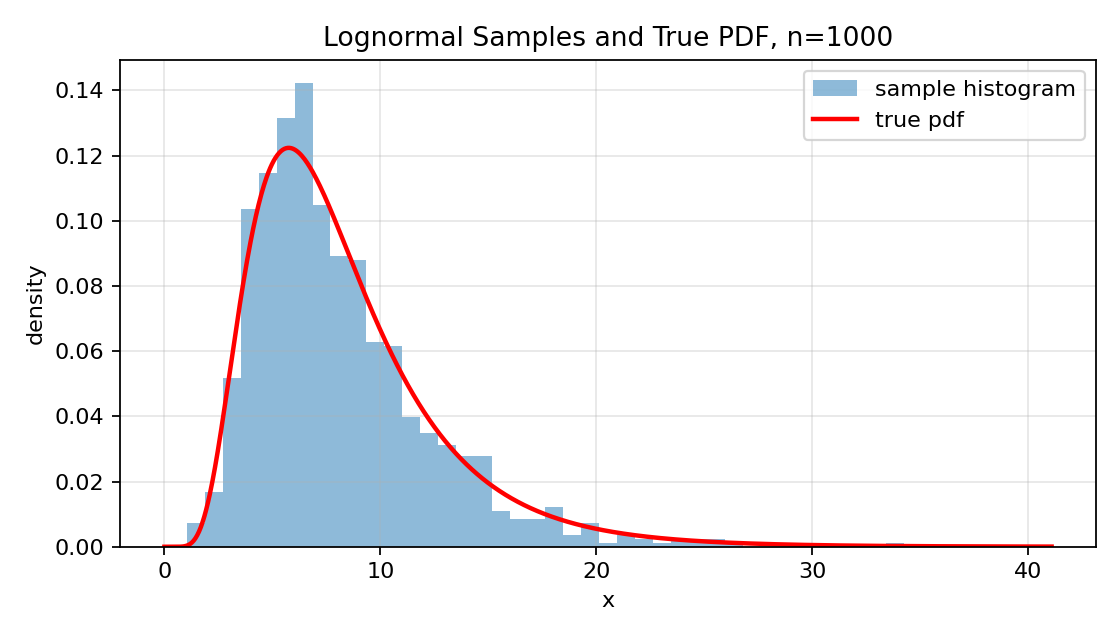
\includegraphics[width=0.72\textwidth]{8_4/kde_part_a_true_pdf.png}
      \caption{对数正态样本直方图与真实概率密度函数}
  \end{figure}

  \item 使用核密度估计时，自动带宽为
  \[
      h=0.812851.
  \]
  KDE 曲线整体上贴近真实的对数正态密度：在主体区域能够估计出单峰形状，在右尾区域由于样本较少，偏差和波动更明显。由于 KDE 使用对称高斯核，而真实分布只在 $x>0$ 上有密度，所以靠近 $0$ 的位置可能存在边界偏差；不过本题参数下主要概率质量远离 $0$，边界影响不明显。

  \begin{figure}[htbp]
      \centering
      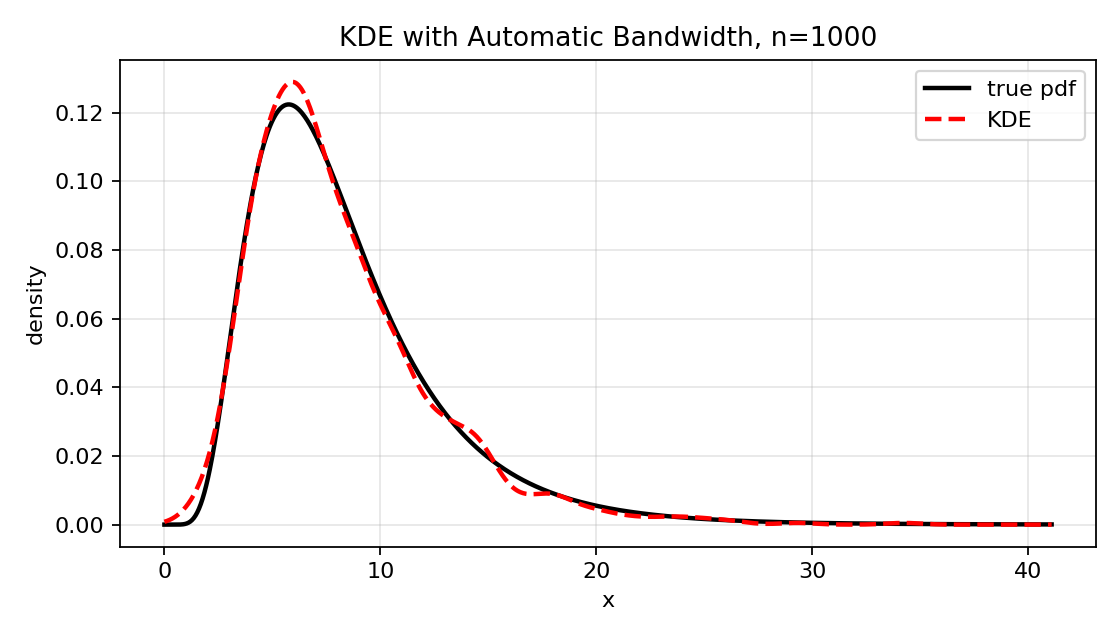
\includegraphics[width=0.72\textwidth]{8_4/kde_part_b_auto_bandwidth.png}
      \caption{自动带宽下的 KDE 与真实密度对比}
  \end{figure}

  \item 带宽取 $0.2$ 时，核函数很窄，估计曲线会紧跟样本点变化，表现为局部尖峰较多、曲线较抖。这对应较小偏差和较大方差，容易过拟合样本随机波动。

  带宽取 $5$ 时，核函数很宽，估计曲线会被强烈平滑，峰值被压低，分布主体被拉宽，右尾和左侧区域可能被过度抬高。这对应较大偏差和较小方差，容易欠拟合真实密度形状。

  因此，KDE 带宽控制的是偏差--方差折中：带宽太小，估计方差大；带宽太大，估计偏差大。较合适的带宽应使曲线既能保持对数正态分布的单峰和右偏特征，又不过度追随样本噪声。

  \begin{figure}[htbp]
      \centering
      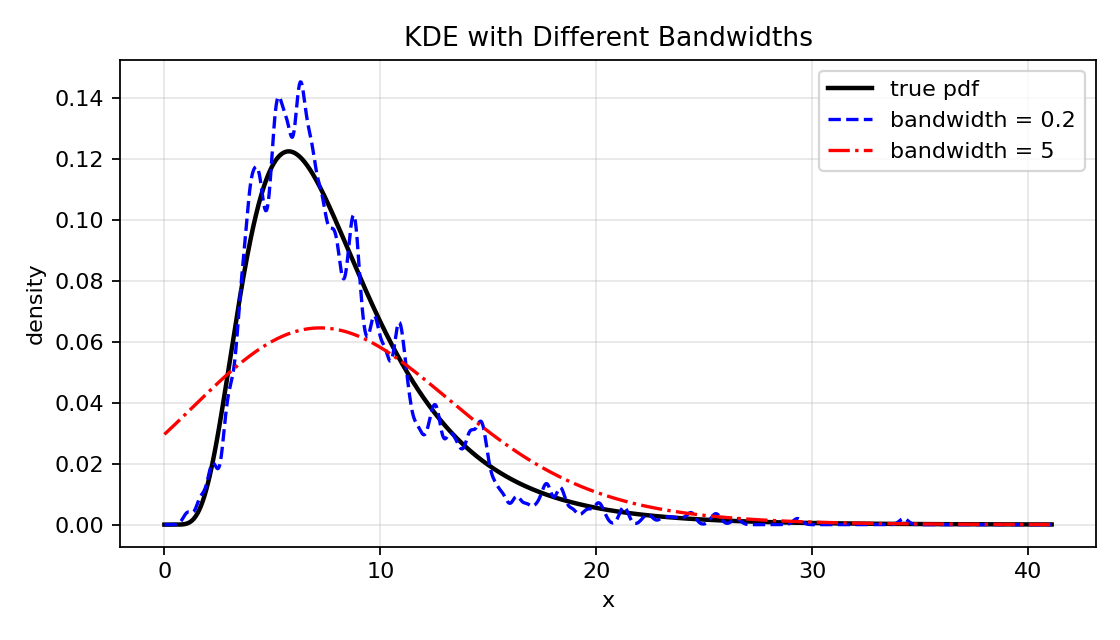
\includegraphics[width=0.72\textwidth]{8_4/kde_part_c_bandwidth_compare.png}
      \caption{不同带宽下 KDE 曲线的比较}
  \end{figure}

  \item 若样本数增加到 $10000$ 或 $100000$，实验得到的自动带宽为
  \[
      \begin{array}{c|ccc}
      n & 1000 & 10000 & 100000\\
      \hline
      h & 0.899396 & 0.548900 & 0.340729
      \end{array}
  \]
  可以看到，随着样本数增加，自动选择的带宽逐渐变小。直观原因是样本越多，局部区域内可用于估计的样本也越多，因此可以使用更窄的核来刻画密度细节，同时仍保持较小方差。许多核密度估计带宽准则具有近似形式
  \[
      h\propto n^{-1/5},
  \]
  因而 $n$ 增大时 $h$ 逐渐减小。例如样本数从 $1000$ 增加到 $10000$，带宽大约乘以
  \[
      \left(\frac{10000}{1000}\right)^{-1/5}=10^{-1/5}\approx0.631;
  \]
  从 $1000$ 增加到 $100000$，带宽大约乘以
  \[
      \left(\frac{100000}{1000}\right)^{-1/5}=100^{-1/5}\approx0.398.
  \]
  因此样本越多，KDE 曲线一般越接近真实密度，随机波动减小，自动带宽也会变小以提高分辨率。

  \begin{figure}[htbp]
      \centering
      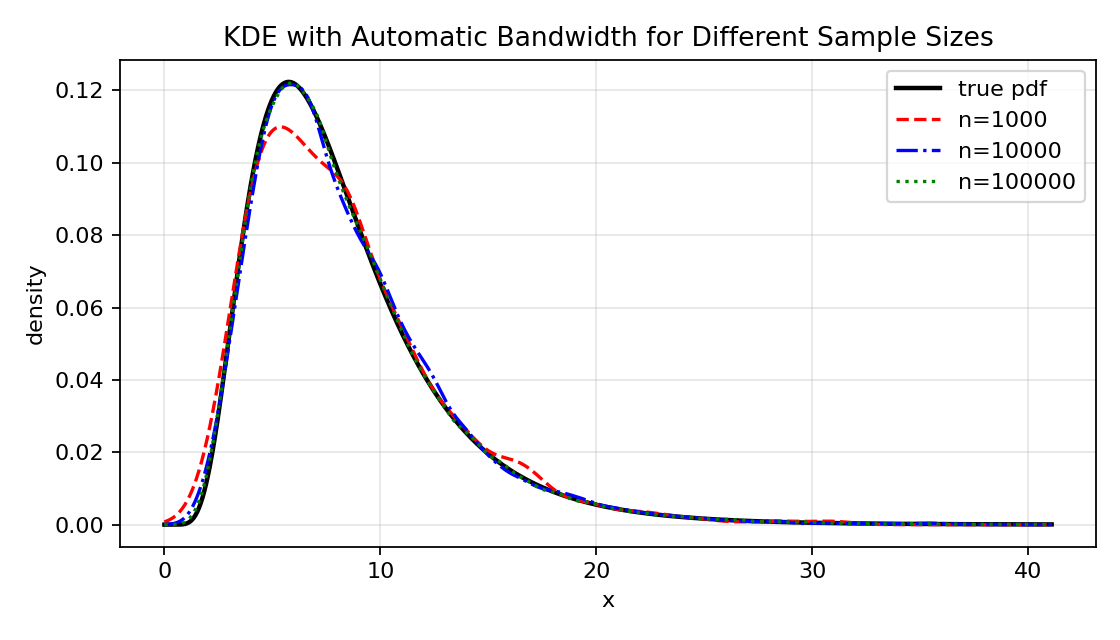
\includegraphics[width=0.72\textwidth]{8_4/kde_part_d_sample_size_compare.png}
      \caption{不同样本数下自动带宽 KDE 的比较}
  \end{figure}
\end{enumerate}

\subsection*{习题 8.6}

两类高斯条件分布为
\[
    p(x\mid y=i)=\Normal(\mu_i,\Sigma),\qquad i=1,2,
\]
且先验相同：
\[
    \Prb(y=1)=\Prb(y=2)=0.5.
\]
在 $0$-$1$ 损失下，Bayes 决策为选择后验概率较大的类别。由于先验相同，只需比较类条件密度：
\[
    \log p(x\mid y=1)-\log p(x\mid y=2)>0.
\]
高斯对数密度中与类别无关的常数会抵消，因此
\begin{align*}
    &-\frac12(x-\mu_1)^T\Sigma^{-1}(x-\mu_1)
    +\frac12(x-\mu_2)^T\Sigma^{-1}(x-\mu_2)>0\\
    \Longleftrightarrow\quad
    &x^T\Sigma^{-1}(\mu_1-\mu_2)
    -\frac12\mu_1^T\Sigma^{-1}\mu_1
    +\frac12\mu_2^T\Sigma^{-1}\mu_2>0.
\end{align*}
所以可写成
\[
    y^*=
    \begin{cases}
    1,& w^Tx+b>0,\\
    2,& w^Tx+b\le0,
    \end{cases}
\]
其中
\[
    w=\Sigma^{-1}(\mu_1-\mu_2),
\]
\[
    b=-\frac12\mu_1^T\Sigma^{-1}\mu_1
      +\frac12\mu_2^T\Sigma^{-1}\mu_2.
\]
若先验不相等，只需在 $b$ 中额外加上 $\log\frac{\Prb(y=1)}{\Prb(y=2)}$。

\section*{第九章 线性代数基础}

\subsection*{习题 9.3}

要证明当 $0<p<q$ 时，
\[
    \|x\|_p
    =
    \left(\sum_{i=1}^d |x_i|^p\right)^{1/p}
    \ge
    \left(\sum_{i=1}^d |x_i|^q\right)^{1/q}
    =
    \|x\|_q.
\]

\begin{enumerate}
  \item 若 $x_i\ge0$，则 $|x_i|=x_i$，原式直接化为
  \[
      (x_1^p+x_2^p+\cdots+x_d^p)^{1/p}
      \ge
      (x_1^q+x_2^q+\cdots+x_d^q)^{1/q}.
  \]

  \item 令
  \[
      r=\frac{q}{p}>1,\qquad y_i=x_i^p.
  \]
  则 $x_i^q=(x_i^p)^{q/p}=y_i^r$。所以
  \[
      (x_1^p+\cdots+x_d^p)^{1/p}
      \ge
      (x_1^q+\cdots+x_d^q)^{1/q}
  \]
  两边取 $p$ 次方，等价于
  \[
      y_1+\cdots+y_d
      \ge
      (y_1^r+\cdots+y_d^r)^{1/r}.
  \]
  再取 $r$ 次方，等价于
  \[
      (y_1+\cdots+y_d)^r
      \ge
      y_1^r+\cdots+y_d^r.
  \]

  \item 证明对 $r>1$、$y_i\ge0$，
  \[
      (y_1+\cdots+y_d)^r\ge y_1^r+\cdots+y_d^r.
  \]
  当 $d=2$ 时，若 $a,b\ge0$，则
  \[
      (a+b)^r=a^r\left(1+\frac{b}{a}\right)^r
  \]
  在 $a>0$ 时成立。因为函数 $(1+t)^r$ 在 $t\ge0$ 上满足
  \[
      (1+t)^r\ge 1+t^r,
  \]
  故 $(a+b)^r\ge a^r+b^r$；$a=0$ 时显然成立。

  对 $d>2$ 使用归纳法。假设对 $d-1$ 个非负数成立，则
  \[
      (y_1+\cdots+y_d)^r
      =
      ((y_1+\cdots+y_{d-1})+y_d)^r
      \ge
      (y_1+\cdots+y_{d-1})^r+y_d^r.
  \]
  再由归纳假设，
  \[
      (y_1+\cdots+y_{d-1})^r
      \ge y_1^r+\cdots+y_{d-1}^r.
  \]
  因而
  \[
      (y_1+\cdots+y_d)^r
      \ge y_1^r+\cdots+y_d^r.
  \]

  \item 下面不再使用前面两步中的简化假设和变量替换，直接证明一般实向量情形。若 $x=0$，则任意 $p>0$ 都有 $\|x\|_p=0$，结论显然成立。下面设 $x\ne0$。

  记
  \[
      S(p)=\sum_{i=1}^d |x_i|^p,\qquad
      g(p)=\log\|x\|_p=\frac{1}{p}\log S(p).
  \]
  只需证明 $g'(p)\le0$，因为这说明 $\log\|x\|_p$ 关于 $p$ 单调不增，从而 $\|x\|_p$ 关于 $p$ 单调不增。

  先处理所有非零分量。设 $a_i=|x_i|>0$，并定义权重
  \[
      w_i=\frac{a_i^p}{\sum_{j=1}^d a_j^p},
      \qquad \sum_{i=1}^d w_i=1,\quad w_i>0.
  \]
  对 $g(p)$ 求导：
  \begin{align*}
      g'(p)
      &=-\frac{1}{p^2}\log S(p)
        +\frac{1}{p}\frac{S'(p)}{S(p)}\\
      &=-\frac{1}{p^2}\log S(p)
        +\frac{1}{p}\sum_{i=1}^d w_i\log a_i.
  \end{align*}
  于是
  \[
      p^2g'(p)
      =
      p\sum_{i=1}^d w_i\log a_i-\log S(p).
  \]
  又因为
  \[
      \log w_i=p\log a_i-\log S(p),
  \]
  所以
  \[
      p\log a_i=\log w_i+\log S(p).
  \]
  代入上式：
  \[
      p^2g'(p)
      =
      \sum_{i=1}^d w_i(\log w_i+\log S(p))-\log S(p)
      =
      \sum_{i=1}^d w_i\log w_i.
  \]
  由于 $0<w_i\le1$，所以 $\log w_i\le0$，从而
  \[
      \sum_{i=1}^d w_i\log w_i\le0.
  \]
  因此
  \[
      g'(p)\le0.
  \]

  若某些分量 $x_i=0$，则这些项对 $S(p)$ 没有贡献，可以只在非零分量集合上定义权重；上述推导不变。若只有一个非零分量，则唯一权重为 $1$，此时 $g'(p)=0$，范数对 $p$ 不变。

  因而对任意实向量 $x\in\mathbb{R}^d$、任意 $0<p<q$，
  \[
      \log\|x\|_p=g(p)\ge g(q)=\log\|x\|_q.
  \]
  由于对数函数单调递增，得到
  \[
      \|x\|_p\ge \|x\|_q,
  \]
  即公式 (9.66) 在不使用前面简化条件的情况下成立。
\end{enumerate}

\subsection*{习题 9.4}

设 $G\in\mathbb{R}^{d\times d}$ 是正定矩阵，定义
\[
    \|x\|_G=\|Gx\|_2,\qquad x\in\mathbb{R}^d.
\]
证明它是向量范数，只需验证范数三条性质。

\begin{enumerate}
  \item 非负性与正定性：
  \[
      \|x\|_G=\|Gx\|_2\ge0.
  \]
  若 $\|x\|_G=0$，则 $\|Gx\|_2=0$，所以 $Gx=0$。正定矩阵必可逆，因此 $x=0$。反之 $x=0$ 时显然 $\|x\|_G=0$。

  \item 齐次性：对任意标量 $a$，
  \[
      \|ax\|_G=\|G(ax)\|_2=\|aGx\|_2=|a|\|Gx\|_2=|a|\|x\|_G.
  \]

  \item 三角不等式：对任意 $x,y$，
  \[
      \|x+y\|_G
      =\|G(x+y)\|_2
      =\|Gx+Gy\|_2
      \le \|Gx\|_2+\|Gy\|_2
      =\|x\|_G+\|y\|_G.
  \]
\end{enumerate}

因此 $\|Gx\|_2$ 是一个有效的向量范数。事实上，这个结论只需要 $G$ 可逆；正定性保证了 $G$ 可逆。

\end{document}
